\documentclass[11pt]{article}
\usepackage{matt}
\begin{document}

\section*{Update for the Week of \today}

\begin{figure}[h]
  \centering
  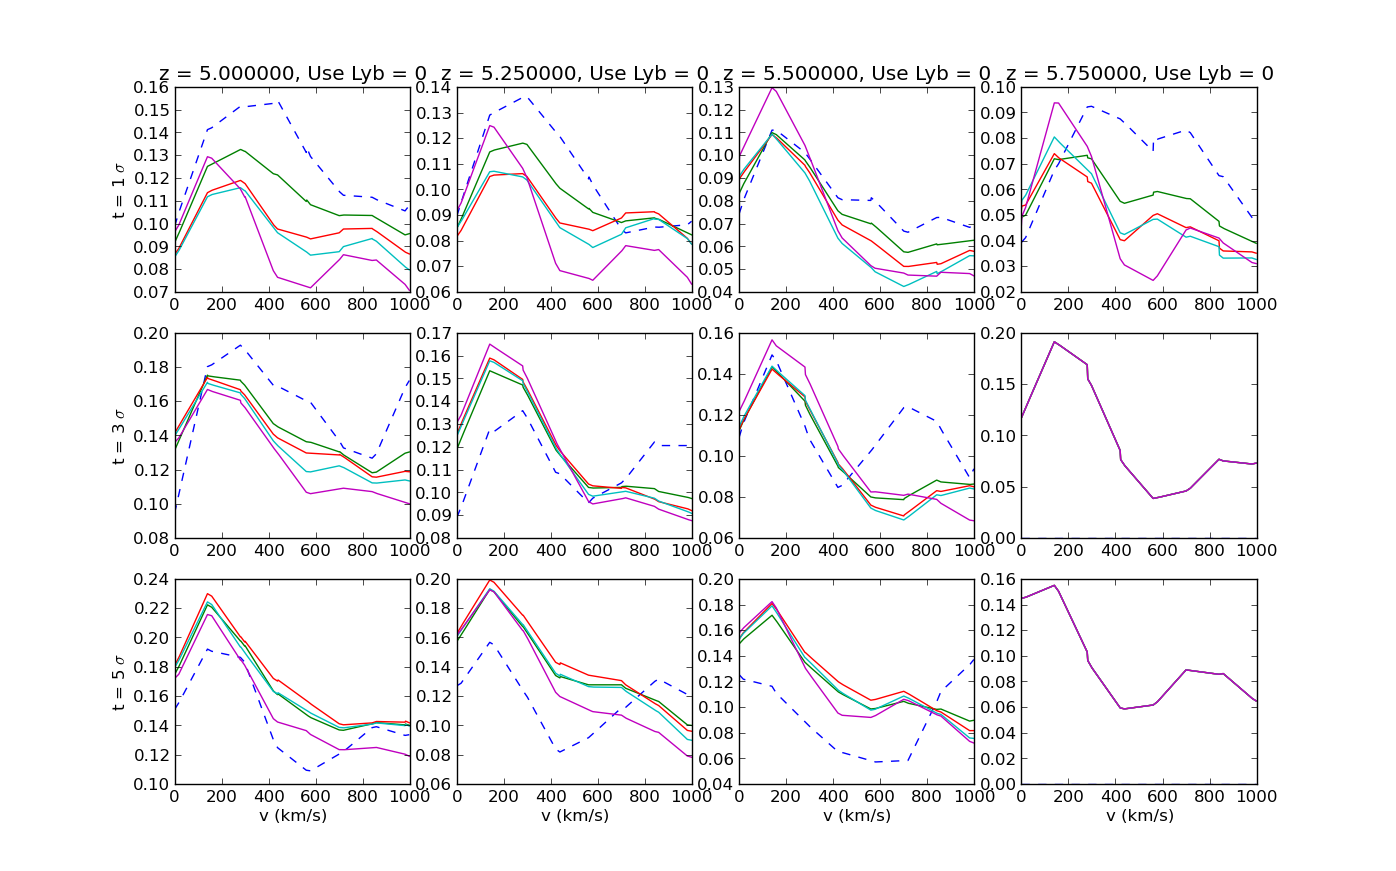
\includegraphics[width=18cm]{gridPlot_CommonRes.png}
  \caption{todo}
  \label{fig:todo}
\end{figure}

\begin{figure}[h]
  \centering
  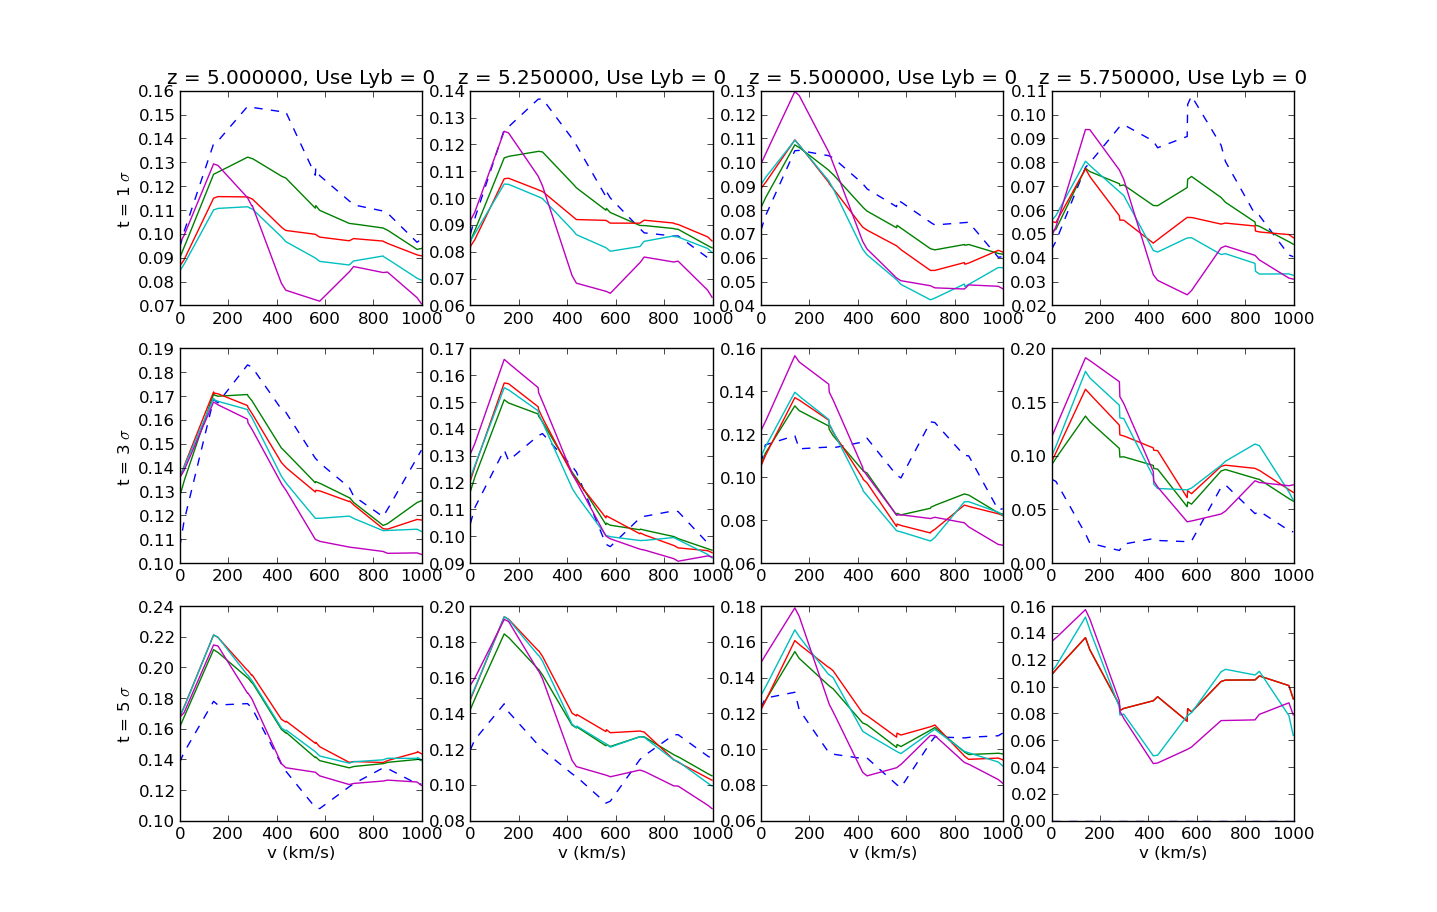
\includegraphics[width=18cm]{gridPlot_CommonRes_AllSpectra.png}
  \caption{todo}
  \label{fig:todo}
\end{figure}

\begin{figure}[h]
\subsubsection*{Suspicious Behavior from $z = 5.99$ Spectrum}
  \centering
  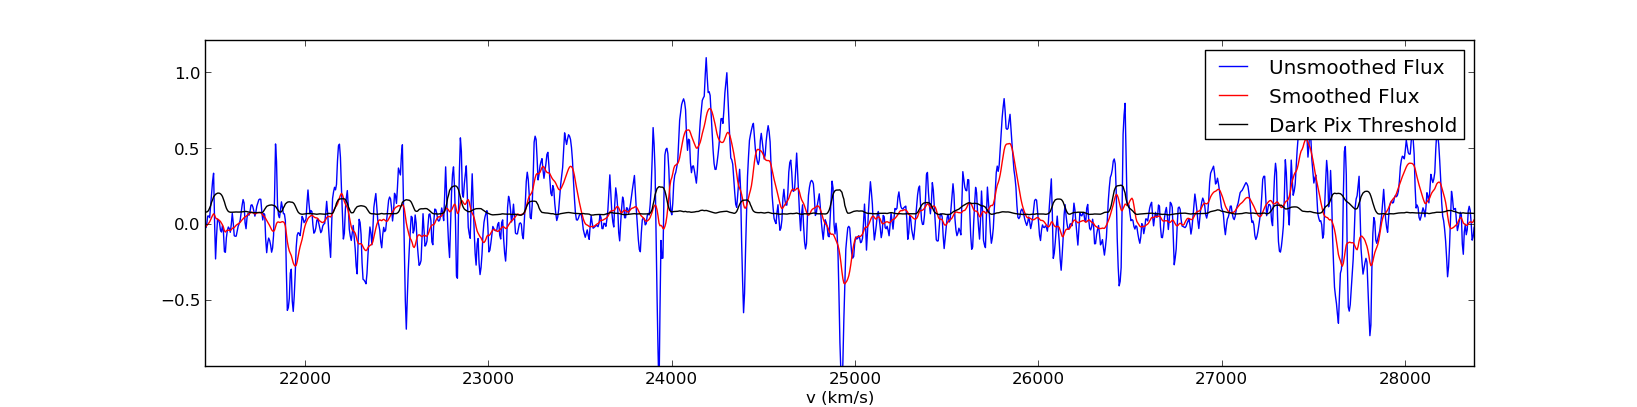
\includegraphics[width=18cm]{z599_Spectra.png}
  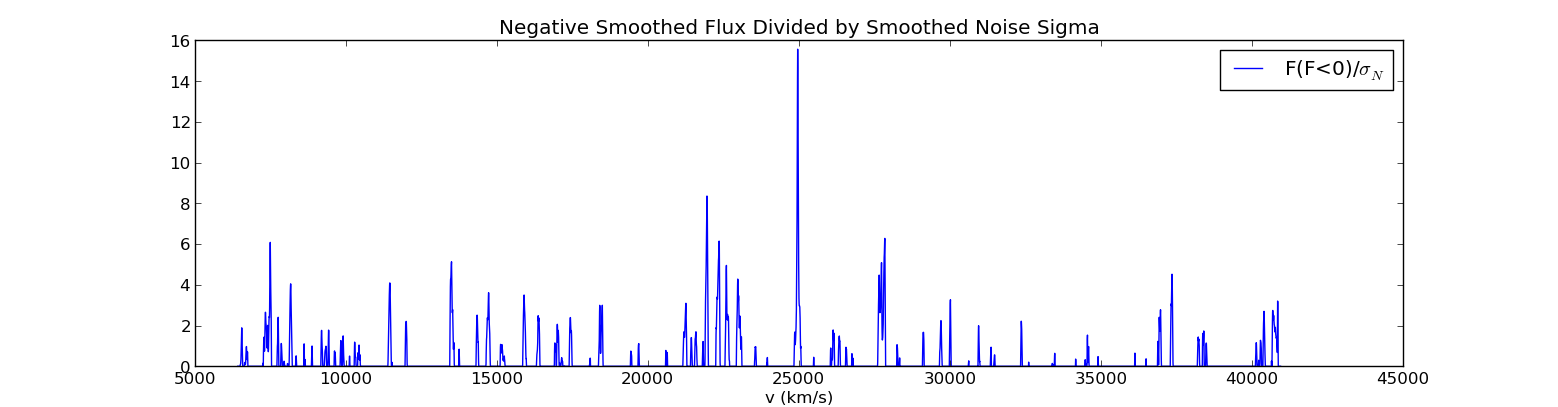
\includegraphics[width=18cm]{z599_NoiseSignificance.png}
  \caption{The top panel shows the unsmoothed spectrum (blue), smoothed spectrum (red) and dark-pixel threshold (black) for the $z = 5.99$ spectrum. The dark-pixel threshold is defined to be $3\tilde{\sigma}_{\text{N}}$. The bottom panel shows negative values in the smoothed spectrum \textit{in units of $\tilde{\sigma}_{\text{N}}$}. From this figure, it seems that negative noise fluctuations in the smoothed spectrum are frequently in excess of $6\tilde{\sigma}_{\text{N}}$.}
  \label{fig:z599}
\end{figure}

\begin{figure}[h]
\subsubsection*{$z = 6.28$ Spectrum}
  \centering
  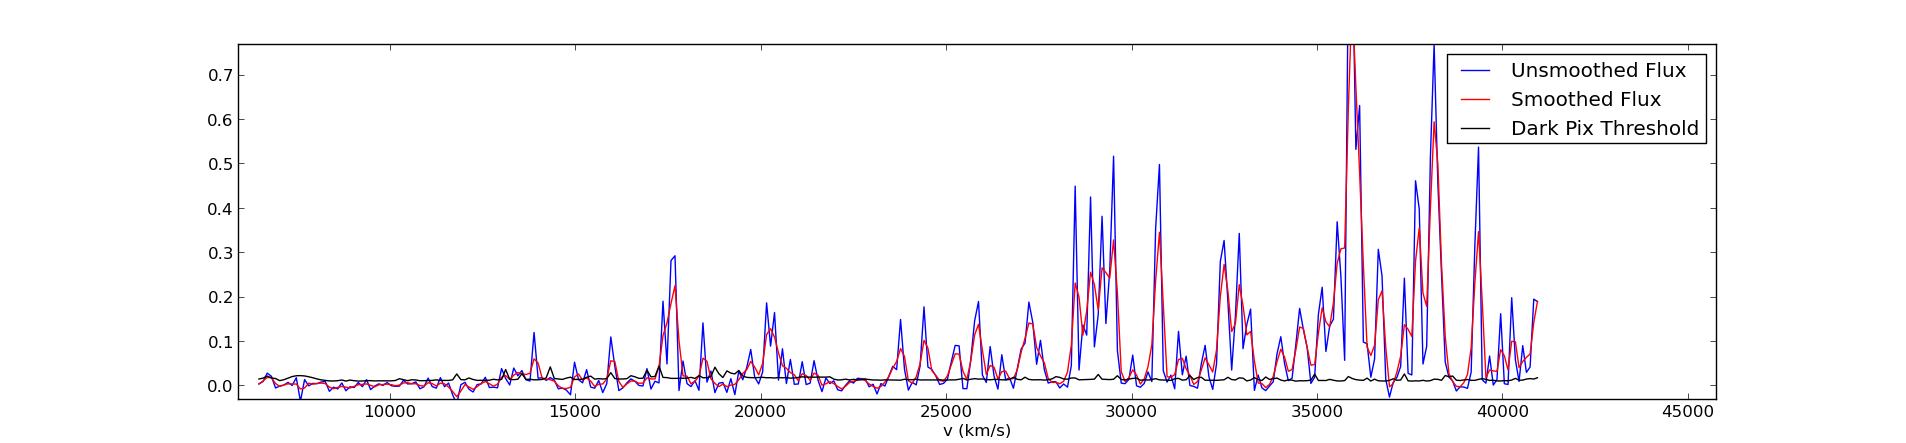
\includegraphics[width=18cm]{z628_Spectra.png}
  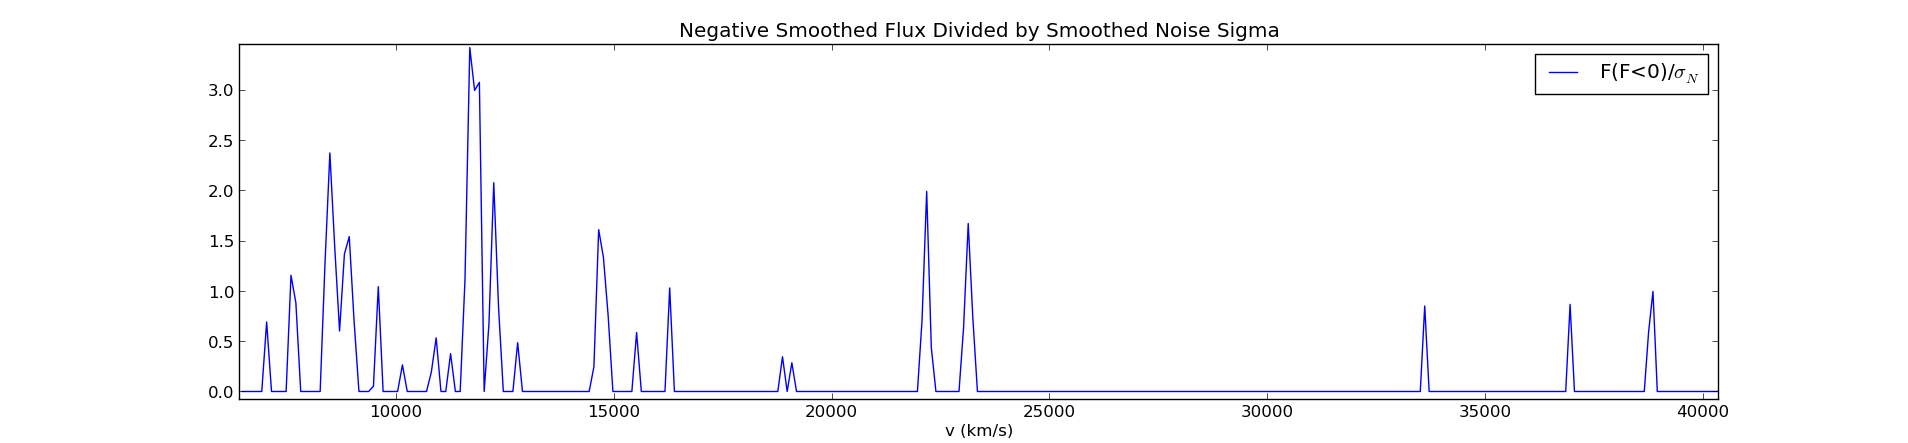
\includegraphics[width=18cm]{z628_NoiseSignificance.png}
  \caption{This figure is the same as Figure \ref{fig:z599}, except for a spectrum with $z_{\text{QSO}} = 6.28$. This spectrum doesn't display suspicious behavior during stacking. It also does not display curiously large downward fluctuations in the noise.}
  \label{fig:todo}
\end{figure}



\end{document}